\documentclass[letterpaper,10pt]{article}

\usepackage{enumitem}
\usepackage{titling}
\usepackage{listings,listings-rust}
\usepackage{url}
\usepackage{soul}
\usepackage{hyperref}
\usepackage{setspace}
\usepackage{subfig}
\usepackage{sectsty}
\usepackage{pdfpages}
\usepackage{colortbl}
\usepackage{multirow}
\usepackage{multicol}
\usepackage{relsize}
\usepackage{amsmath}
\usepackage{wasysym}
\usepackage{fancyvrb}
\usepackage[yyyymmdd]{datetime}
\usepackage{amsmath,amssymb,amsthm,graphicx,xspace}
\usepackage[titlenotnumbered,noend,noline]{algorithm2e}
\usepackage[compact]{titlesec}
\usepackage{XCharter}
\usepackage[T1]{fontenc}
\usepackage[scaled]{beramono}
\usepackage[normalem]{ulem}
\usepackage{booktabs}
\usepackage{tikz}
\usetikzlibrary{arrows.meta,automata,shapes,trees,matrix,chains,scopes,positioning,calc,decorations.pathreplacing}
\tikzstyle{block} = [rectangle, draw, fill=blue!20, 
    text width=2.5em, text centered, rounded corners, minimum height=2em]
\tikzstyle{bw} = [rectangle, draw, fill=blue!20, 
    text width=4em, text centered, rounded corners, minimum height=2em]

\definecolor{namerow}{cmyk}{.40,.40,.40,.40}
\definecolor{namecol}{cmyk}{.40,.40,.40,.40}
\renewcommand{\dateseparator}{-}

\let\LaTeXtitle\title
\renewcommand{\title}[1]{\LaTeXtitle{\textsf{#1}}}

\lstset{basicstyle=\footnotesize\ttfamily,breaklines=true}

\newcommand{\CPP}{C\nolinebreak\hspace{-.05em}\raisebox{.4ex}{\tiny\bf +}\nolinebreak\hspace{-.10em}\raisebox{.4ex}{\tiny\bf +}}
\def\CPP{{C\nolinebreak[4]\hspace{-.05em}\raisebox{.4ex}{\tiny\bf ++}}}

\newcommand{\handout}[5]{
  \noindent
  \begin{center}
  \framebox{
    \vbox{
      \hbox to 5.78in { {\bf ECE459: Programming for Performance } \hfill #2 }
      \vspace{4mm}
      \hbox to 5.78in { {\Large \hfill #4  \hfill} }
      \vspace{2mm}
      \hbox to 5.78in { {\em #3 \hfill \today} }
    }
  }
  \end{center}
  \vspace*{4mm}
}

\newcommand{\lecture}[3]{\handout{#1}{#2}{#3}{Lecture#1}}
\newcommand{\tuple}[1]{\ensuremath{\left\langle #1 \right\rangle}\xspace}

\addtolength{\oddsidemargin}{-1.000in}
\addtolength{\evensidemargin}{-0.500in}
\addtolength{\textwidth}{2.0in}
\addtolength{\topmargin}{-1.000in}
\addtolength{\textheight}{1.75in}
\addtolength{\parskip}{\baselineskip}
\setlength{\parindent}{0in}
\renewcommand{\baselinestretch}{1.5}
\newcommand{\term}{Winter 2020}

\singlespace


\begin{document}

\lecture{26 --- Liar, Liar}{\term}{Patrick Lam \& Jeff Zarnett}

\section*{Lies about Calling Context}

Let's open with a video that illustrates one of the problems with sampling-based profiling:

\begin{center}
	\url{https://www.youtube.com/watch?v=jQDjJRYmeWg}
\end{center}

The video's not fake; it's a real helicopter and it's really flying. What's happening, however, is that the camera is taking images at some multiple of the frequency of the blade rotation speed so it gives the illusion that the blades are not spinning at all. This is a sampling problem, and you see the same problem in car commercials on TV where it looks like the wheels are spinning backwards. They're not, but the sampling effect of the camera can make it look that way.

Some profiler results are real.  Other results are interpolated, and
perhaps wrong. Who can we trust? We'll start by talking about gprof and callgrind/KCacheGrind. The reference for this part of the lecture is a blog post by Yossi Kreinin~\cite{lies}.

\paragraph{Running Example.} Consider the following code.

\begin{lstlisting}
void work(int n) {
  volatile int i=0; //don't optimize away
  while(i++ < n);
}
void easy() { work(1000); }
void hard() { work(1000*1000*1000); }
int main() { easy(); hard(); }
\end{lstlisting}

We see that there is a worker function whose runtime depends on its input.
Function {\tt easy} calls the worker function with a small input, and {\tt hard} calls
it with a large input. So we expect most of the time should be spent in the \texttt{hard} function, right? 
Profiling yields:
\begin{verbatim}
[plam@lynch L27]\$ gprof ./try gmon.out
Flat profile:

Each sample counts as 0.01 seconds.
  \%   cumulative   self              self     total           
 time   seconds   seconds    calls  ms/call  ms/call  name    
101.30      1.68     1.68        2   840.78   840.78  work
  0.00      1.68     0.00        1     0.00  {840.78}  easy
  0.00      1.68     0.00        1     0.00  {840.78}  hard
\end{verbatim}
%$
Most of the profiler output is just fine. But there are lies in the
``total ms/call'' column. The call to {\tt easy} takes about 0 seconds,
while that to {\tt hard} takes 1.68s. Less importantly, the total ms/call for
{\tt work} is indeed an average, but that hides the variance between runtimes.

\paragraph{Why?} To make any sense of the lies, we need to understand how {\tt gprof} works.
It uses two standard-library functions: {\bf profil()} and {\bf mcount()}.

\begin{itemize}
\item {\bf profil()}: asks glibc to record which instruction 
  is currently executing (100$\times$/second).
\item {\bf mcount()}: records call graph edges; called by {\tt -pg} instrumentation.
\end{itemize}

Hence, {\bf profil} information is statistical, while {\bf mcount}
information is exact.  Bringing that information back to the profiler
output columns, we can see that the ``calls'' column is reliable; the
``self seconds'' column is sampled, but reasonably accurate here; and
the ``total ms/call'' is interpolated, and we deceived it in this
contrived example. How is that?

gprof sees:
\begin{itemize}
    \item a total of 1.68s in {\tt work};
    \item 1 call to {\tt work} from {\tt easy}; and
    \item 1 call to {\tt work} from {\tt hard}.
\end{itemize}
All of these numbers are reliable. However, gprof draws the unreliable inference that
both {\tt easy}, {\tt hard} cause 840ms of {\tt work} time. How did we get here? Well, gprof used some correct data: 3.84 seconds spent in \texttt{work}, divides it between \texttt{easy} and \texttt{hard}, each of which \texttt{mcount} reported was called once, and gets 1.92. So we got a bogus result using correct 

This is wrong. {\tt work} takes 1000000$\times$ longer when called from {\tt hard}!


The following results from gprof are suspect:
\begin{itemize}
  \item contribution of children to parents;
  \item total runtime spent in self+children;
  \item etc.
\end{itemize}

\paragraph{When are call graph edges right?}
Two cases:
    \begin{itemize}
    \item functions with only one caller
      (e.g. {\tt f()} only called by {\tt g()}); or,
    \item functions which always take the same time to complete
      (e.g. {\tt rand()}).
    \end{itemize}

On the other hand, results for any function whose running time depends on its inputs,
and which is called from multiple contexts, are sketchy.

\subsection*{callgrind/KCacheGrind}
Next, we'll talk about callgrind/KCacheGrind. Like our old friends memcheck, hell grind, and cachegrind, callgrind is part of valgrind, and runs the program under an x86 JIT.  KCacheGrind is a frontend to callgrind. callgrind gives better information, but imposes
more overhead.

\newpage
KCacheGrind works properly on the earlier running example:

\begin{center}
  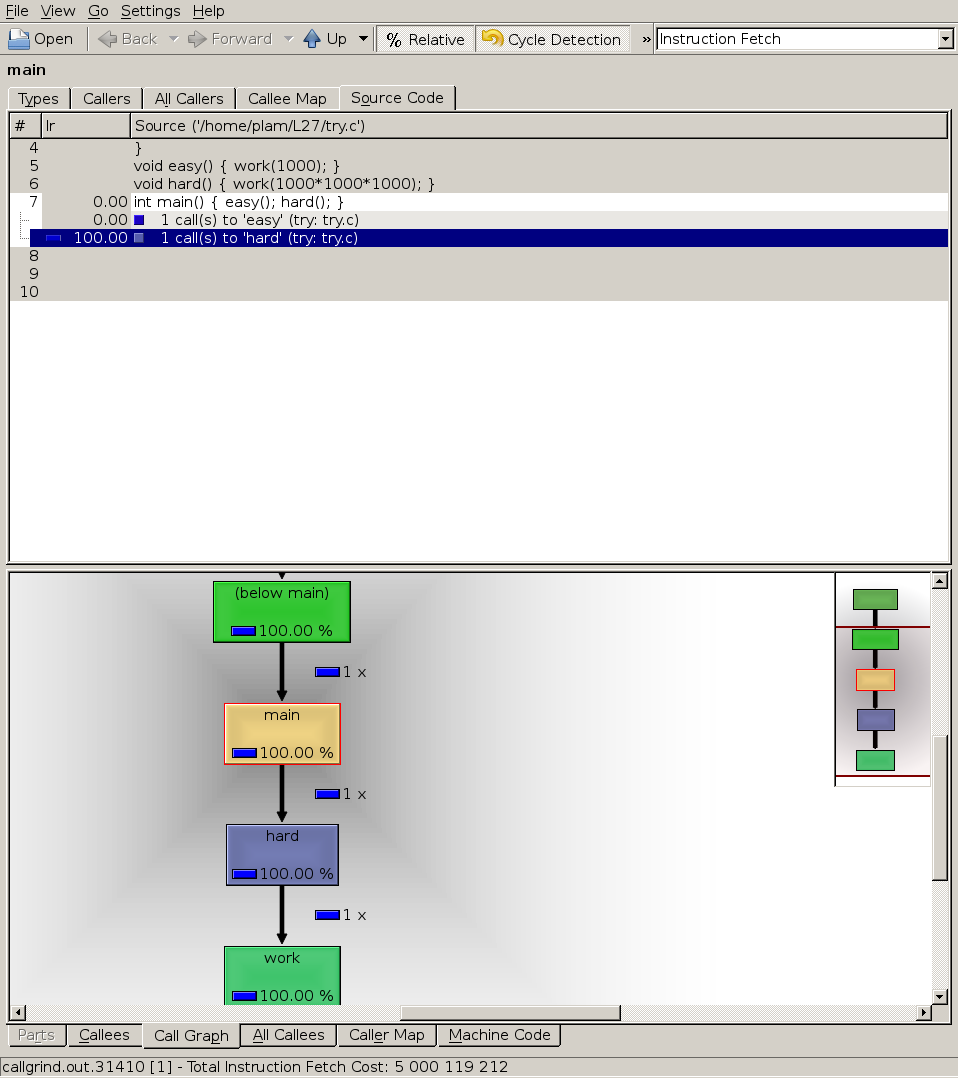
\includegraphics[width=.4\textwidth]{images/kcachegrind}
\end{center}

It properly reports that {\tt hard} takes all the time.
But we can still deceive it.

\paragraph{More Complex Example.} Let's look at this example.

\begin{minipage}{.4\textwidth}
\begin{lstlisting}[basicstyle=\scriptsize]
void worker1(int n) {
  volatile int i=0;
  while(i++<n);
}
void worker2(int n) {
  volatile int i=0;
  while(i++<n);
}
void manager(int n1, int n2) {
  worker1(n1);
  worker2(n2);
}
\end{lstlisting}
\end{minipage}
\begin{minipage}{.4\textwidth}
\begin{lstlisting}[basicstyle=\scriptsize]
void project1() {
  manager(1000, 1000000);
}
void project2() {
  manager(1000000, 1000);
}
int main() {
  project1();
  project2();
}
\end{lstlisting}
\end{minipage}

Now, {\tt worker2} takes all the time in {\tt project1},
and {\tt worker1} takes all the time in {\tt project2}.

Let's see how KCacheGrind does on this example.

\begin{center}
  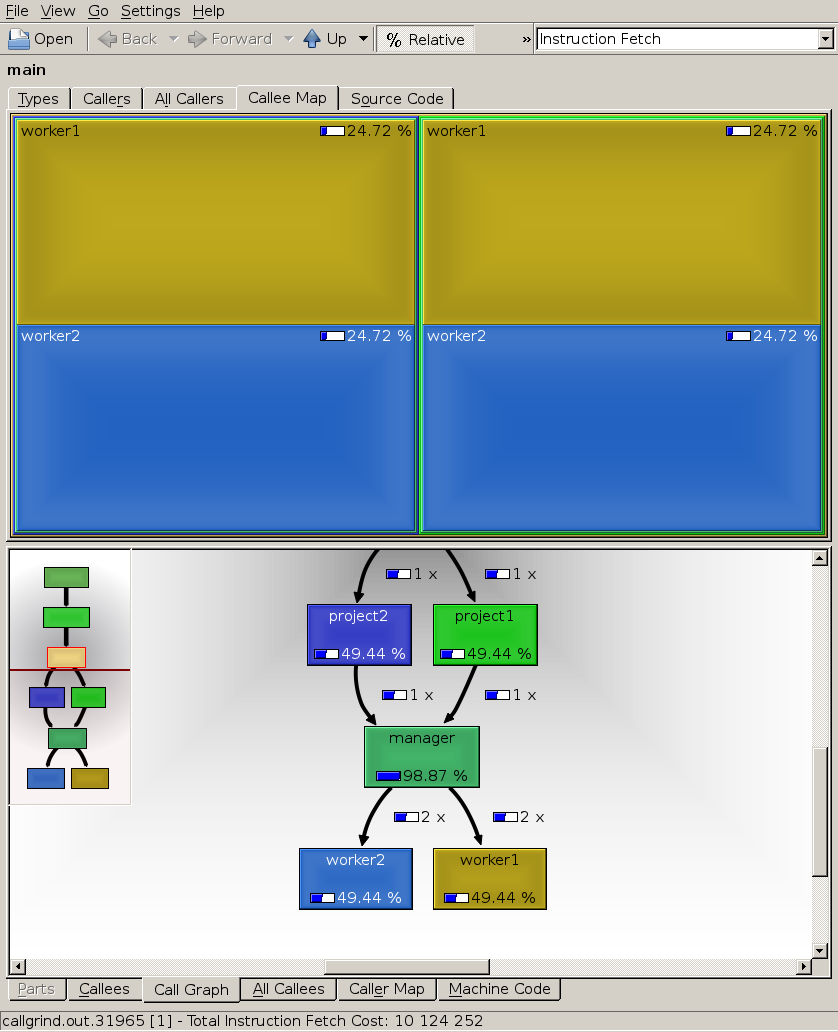
\includegraphics[width=.25\textwidth]{images/kcachegrind2}
\end{center}


The call graph, on the bottom, shows that 
{\tt worker1} and {\tt worker2} do each take about 50\% of time.
So do {\tt project2} and {\tt project1}. This is fine.
(I think gprof would correctly interpolate that too.)

However, KCacheGrind also lies, in the report on top. It is saying
that {\tt worker1} and {\tt worker2} doing half the work in each
project.  That's not what the code says. Why is it lying?

\begin{itemize}
\item gprof reports time spent in {\tt f()} and {\tt g()},
and how many times {\tt f()} calls {\tt g()}.
\item callgrind also reports 
time spent  in {\tt g()} when called from {\tt f()}, i.e. some calling-context information.
\item callgrind does \emph{not} report time spent in {\tt g()} when
     called from {\tt f()} when called from {\tt h()}.
     We don't get the {\tt project1} to {\tt manager} to {\tt worker1} link.
     (We have Edges but need Edge-Pairs).
\end{itemize}

\paragraph{Summary.} We've seen that some profiler results are exact;
some results are sampled; and some results are interpolated. If you understand the tool, you understand where it can go
wrong. 

Understand your tools!

\section*{Lies from Metrics}
While app-specific metrics can lie too, mostly we'll talk about CPU
perf counters today.

The reference here is a blog post by Paul Khuong~\cite{metrics}.

This goes back to {\tt mfence}, which we've seen before. It is used, for instance, in
spinlock implementations. Khuong found that his profiles said that spinlocking didn't take much time.
But empirically: eliminating spinlocks = better than expected! Hmm.

The next step is (as we do in this course) to create microbenchmarks to better understand what's
going on. The microbenchmark contained memory accesses to uncached locations, or computations,
surrounded by store pairs/mfence/locks. He used perf to evaluate the impact of mfence vs lock.

{\scriptsize
\begin{lstlisting}
# for locks:
$ perf annotate -s cache_misses
[...]
    0.06 :        4006b0:       and    %rdx,%r10
    0.00 :        4006b3:       add    $0x1,%r9
    ;; random (out of last level cache) read
    0.00 :        4006b7:       mov    (%rsi,%r10,8),%rbp
   30.37 :        4006bb:       mov    %rcx,%r10
    ;; foo is cached, to simulate our internal lock
    0.12 :        4006be:       mov    %r9,0x200fbb(%rip)
    0.00 :        4006c5:       shl    $0x17,%r10
    [... Skipping arithmetic with < 1% weight in the profile]
    ;; locked increment of an in-cache "lock" byte
    1.00 :        4006e7:       lock incb 0x200d92(%rip)
   21.57 :        4006ee:       add    $0x1,%rax
    [...]
    ;; random out of cache read
    0.00 :        400704:       xor    (%rsi,%r10,8),%rbp
   21.99 :        400708:       xor    %r9,%r8
    [...]
    ;; locked in-cache decrement
    0.00 :        400729:       lock decb 0x200d50(%rip)
   18.61 :        400730:       add    $0x1,%rax
    [...]
    0.92 :        400755:       jne    4006b0 <cache_misses+0x30>
\end{lstlisting}
}

We can see that in the lock situation, reads take 30 + 22 = 52\% of runtime,
while locks take 19 + 21 = 40\% of runtime.

{\scriptsize
\begin{lstlisting}
# for mfence:
$ perf annotate -s cache_misses
[...]
    0.00 :        4006b0:       and    %rdx,%r10
    0.00 :        4006b3:       add    $0x1,%r9
    ;; random read
    0.00 :        4006b7:       mov    (%rsi,%r10,8),%rbp
   42.04 :        4006bb:       mov    %rcx,%r10
    ;; store to cached memory (lock word)
    0.00 :        4006be:       mov    %r9,0x200fbb(%rip)
    [...]
    0.20 :        4006e7:       mfence 
    5.26 :        4006ea:       add    $0x1,%rax
    [...]
    ;; random read
    0.19 :        400700:       xor    (%rsi,%r10,8),%rbp
   43.13 :        400704:       xor    %r9,%r8
    [...]
    0.00 :        400725:       mfence 
    4.96 :        400728:       add    $0x1,%rax
    0.92 :        40072c:       add    $0x1,%rax
    [...]
    0.36 :        40074d:       jne    4006b0 <cache_misses+0x30>
\end{lstlisting}
}
Looks like the reads take 85\% of runtime,
while the mfence takes 15\% of runtime.

Metrics lie, though, and when you focus on the metrics as opposed to what you
actually care about, it's easy to be led astray.

In this case, what we actually care about is the total \# of cycles.

    \begin{tabular}{lr}
    No atomic/fence:& 2.81e9 cycles\\
    lock inc/dec: & 3.66e9 cycles\\
    mfence: & 19.60e9 cycles
    \end{tabular}

That 15\% number is a total lie.
Profilers, even using CPU expense counts, drastically underestimate the impact of mfence,
and overestimate the impact of locks.

This is because mfence causes a pipeline flush, and the resulting 
costs get attributed to instructions being flushed, not to the mfence itself.


\section*{The Long Tail}

Our source here is the blog post by Dan Luu~\cite{perf-tracing}. Suppose we have a task that's going to get distributed over multiple computers (like a search). If we look at the latency distribution, the problem is mostly that we see a long tail of events and when we are doing a computation or search where we need all the results, we can only go as the slowest step. Let's take a look at a histogram of disk read latencies, where we are performing a 64 kB read, also from that source:

\begin{center}
	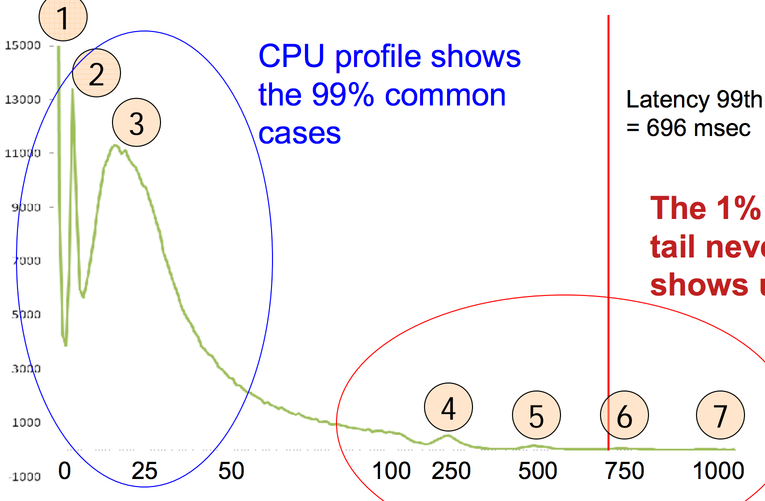
\includegraphics[width=0.65\textwidth]{images/disk_tail.png}
\end{center}

Let's break it down. Peak 1 corresponds to something cached in RAM - best case scenario. Peak 2 is at around 3ms, which is too fast for spinning and seeking magnetic hard disks, but it's fast enough for reading something from the disk cache via the PCI-Express interface. Peak 3 is obviously disk seek and read times, somewhere around 25ms. 

These numbers don't look terrible, except for the fact that we have peaks at 250, 500, 750, and 1000 ms and the 99th percentile is some 696ms which is a very, very long time. Sampling profilers are not very good at finding these things, because they throw everything into various buckets and therefore we get averages. The averages are misleading, though, because we have these weird outliers that take dramatically longer. Averages are nice as long as our data is also reasonably ``nice''.

So what actually happened? Well, from~\cite{perf-tracing}: The investigator found out that the cause was kernel throttling of the CPU for processes that went beyond their usage quota. To enforce the quota, the kernel puts all of the relevant threads to sleep until the next multiple of a quarter second. When the quarter-second hand of the clock rolls around, it wakes up all the threads, and if those threads are still using too much CPU, the threads get put back to sleep for another quarter second. The phase change out of this mode happens when, by happenstance, there aren�t too many requests in a quarter second interval and the kernel stops throttling the threads. After finding the cause, an engineer found that this was happening on 25\% of disk servers at Google, for an average of half an hour a day, with periods of high latency as long as 23 hours. This had been happening for three years.

Further limitations of sampling profilers emerge, as demonstrated in this graph, also from~\cite{perf-tracing}, showing the data we get out of our sampling profiler if we take a look at Lucene (a search indexer):

\begin{center}
	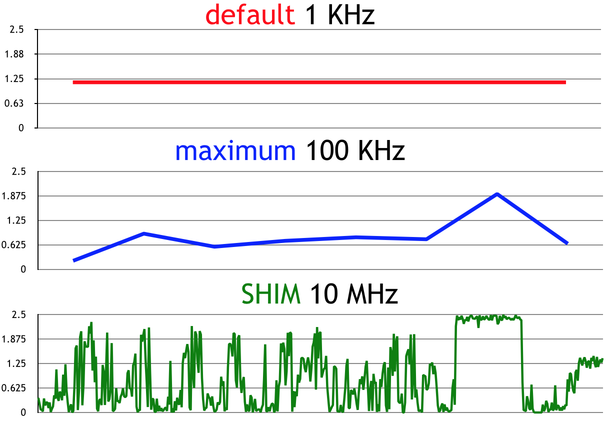
\includegraphics[width=0.5\textwidth]{images/perf-sample.png}
\end{center}

So at the default sampling interval for perf we see... nothing interesting whatsoever. If we bump up to the max sampling frequency of perf, we get a moderately more interesting graph, but not much. If we use a different tool and can sample at a dramatically higher rate, then we end up with something way more useful. So we're left to wonder why does perf sample so infrequently, and how does SHIM get around this?

Well, for one thing, perf samples are done with interrupts. Processing interrupts takes a fair amount of time and if you crank up the rate of interrupts, before long, you are spending all your time handling the interrupts rather than doing useful work. SHIM gets around this by being more invasive -- it adds some periodically executed code that puts information out whenever there is an appropriate event (e.g., function return). This produces a bunch of data which can be dealt with later to produce something useful.

  \paragraph{Algorithmic profiling.} From the recent research literature,
  {\tt aprof} is another profiling tool.
  \url{https://code.google.com/p/aprof/}
{
  \begin{quote}
  aprof is a Valgrind tool for performance profiling designed to help developers discover hidden asymptotic inefficiencies in the code. From one or more runs of a program, aprof measures how the performance of individual routines scales as a function of the input size, yielding clues to its growth rate and to the "big-O" of the program.
  \end{quote}
  }

\paragraph{Summary} We saw a bunch of lies today: calling-context lies and perf attribution
lies. To avoid being bitten by lies, remember to focus on the metric you actually care about,
and understand how your tools work.


\bibliographystyle{alphaurl}
\bibliography{459}


\end{document}
